% Original vector reconstruction of source Fig.65.1, PDF268.
% Dashed arrows denote complex-scalar charge flow; arrows beside photon waves denote momentum.
% All dimensions are native millimetres; definitions are local to this picture.
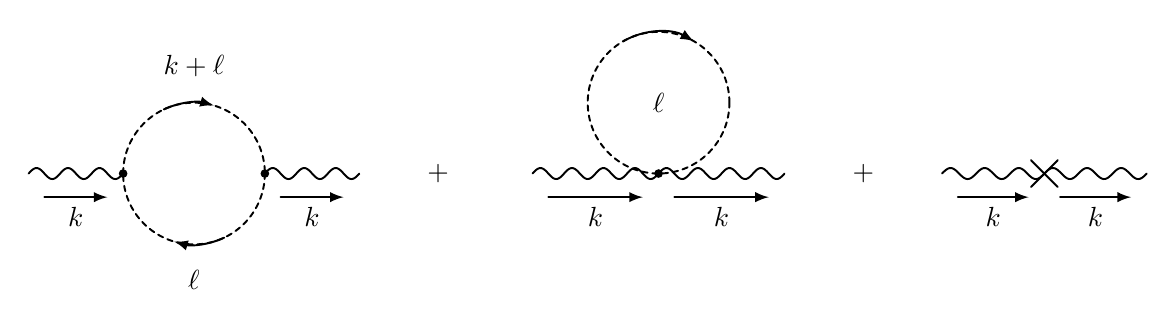
\begin{tikzpicture}[x=1mm,y=1mm,line width=.7pt,>=latex,
 line cap=round,line join=round,font=\fontsize{10}{12}\selectfont,
 scalar/.style={dash pattern=on 2pt off 1.7pt}]
% S65-D001: gL a->vL; gR vR->b; upper scalar vL->vR, lower scalar vR->vL; S=1.
\draw[domain=0:1,samples=101,smooth,variable=\u]
 plot ({0+(12)*\u+(0)*sin(1080*\u)},
       {0+(0)*\u+(0.7)*sin(1080*\u)});
\draw[->] (2,-3)--(10,-3);
\node[below] at (6,-3) {$k$};
\draw[domain=0:1,samples=101,smooth,variable=\u]
 plot ({30+(12)*\u+(0)*sin(1080*\u)},
       {0+(0)*\u+(0.7)*sin(1080*\u)});
\draw[->] (32,-3)--(40,-3);
\node[below] at (36,-3) {$k$};
\draw[scalar] (12,0) arc[start angle=180,end angle=0,radius=9mm];
\draw[->] (17.168,8.1434) arc[start angle=115.2,end angle=73.8,radius=9mm];
\draw[scalar] (30,0) arc[start angle=0,end angle=-180,radius=9mm];
\draw[->] (24.832,-8.1434) arc[start angle=-64.8,end angle=-106.2,radius=9mm];
\node[above] at (21,11) {$k+\ell$};
\node[below] at (21,-11) {$\ell$};
\fill (12,0) circle[radius=.55mm];
\fill (30,0) circle[radius=.55mm];
\node at (52,0) {$+$};
% S65-D002: one oriented scalar self-loop at the seagull, S=1.
\draw[domain=0:1,samples=101,smooth,variable=\u]
 plot ({64+(16)*\u+(0)*sin(1440*\u)},
       {0+(0)*\u+(0.7)*sin(1440*\u)});
\draw[->] (66,-3)--(78,-3);
\node[below] at (72,-3) {$k$};
\draw[domain=0:1,samples=101,smooth,variable=\u]
 plot ({80+(16)*\u+(0)*sin(1440*\u)},
       {0+(0)*\u+(0.7)*sin(1440*\u)});
\draw[->] (82,-3)--(94,-3);
\node[below] at (88,-3) {$k$};
\draw[scalar] (80,9) circle[radius=9mm];
\draw[->] (75.5,16.7942) arc[start angle=120,end angle=60,radius=9mm];
\node at (80,9) {$\ell$};
\fill (80,0) circle[radius=.55mm];
\node at (106,0) {$+$};
% S65-D003: photon two-point counterterm; cross is the only insertion.
\draw[domain=0:1,samples=101,smooth,variable=\u]
 plot ({116+(13)*\u+(0)*sin(1080*\u)},
       {0+(0)*\u+(0.7)*sin(1080*\u)});
\draw[->] (118,-3)--(127,-3);
\node[below] at (122.5,-3) {$k$};
\draw[domain=0:1,samples=101,smooth,variable=\u]
 plot ({129+(13)*\u+(0)*sin(1080*\u)},
       {0+(0)*\u+(0.7)*sin(1080*\u)});
\draw[->] (131,-3)--(140,-3);
\node[below] at (135.5,-3) {$k$};
\draw (127.3,-1.7)--(130.7,1.7);
\draw (127.3,1.7)--(130.7,-1.7);
\end{tikzpicture}
